% Options for packages loaded elsewhere
\PassOptionsToPackage{unicode}{hyperref}
\PassOptionsToPackage{hyphens}{url}
%
\documentclass[
]{article}
\usepackage{lmodern}
\usepackage{amssymb,amsmath}
\usepackage{ifxetex,ifluatex}
\ifnum 0\ifxetex 1\fi\ifluatex 1\fi=0 % if pdftex
  \usepackage[T1]{fontenc}
  \usepackage[utf8]{inputenc}
  \usepackage{textcomp} % provide euro and other symbols
\else % if luatex or xetex
  \usepackage{unicode-math}
  \defaultfontfeatures{Scale=MatchLowercase}
  \defaultfontfeatures[\rmfamily]{Ligatures=TeX,Scale=1}
\fi
% Use upquote if available, for straight quotes in verbatim environments
\IfFileExists{upquote.sty}{\usepackage{upquote}}{}
\IfFileExists{microtype.sty}{% use microtype if available
  \usepackage[]{microtype}
  \UseMicrotypeSet[protrusion]{basicmath} % disable protrusion for tt fonts
}{}
\makeatletter
\@ifundefined{KOMAClassName}{% if non-KOMA class
  \IfFileExists{parskip.sty}{%
    \usepackage{parskip}
  }{% else
    \setlength{\parindent}{0pt}
    \setlength{\parskip}{6pt plus 2pt minus 1pt}}
}{% if KOMA class
  \KOMAoptions{parskip=half}}
\makeatother
\usepackage{xcolor}
\IfFileExists{xurl.sty}{\usepackage{xurl}}{} % add URL line breaks if available
\IfFileExists{bookmark.sty}{\usepackage{bookmark}}{\usepackage{hyperref}}
\hypersetup{
  pdftitle={Creating Learning Curves},
  pdfauthor={Luis H. John, Jenna M. Reps, Peter R. Rijnbeek},
  hidelinks,
  pdfcreator={LaTeX via pandoc}}
\urlstyle{same} % disable monospaced font for URLs
\usepackage[margin=1in]{geometry}
\usepackage{color}
\usepackage{fancyvrb}
\newcommand{\VerbBar}{|}
\newcommand{\VERB}{\Verb[commandchars=\\\{\}]}
\DefineVerbatimEnvironment{Highlighting}{Verbatim}{commandchars=\\\{\}}
% Add ',fontsize=\small' for more characters per line
\usepackage{framed}
\definecolor{shadecolor}{RGB}{248,248,248}
\newenvironment{Shaded}{\begin{snugshade}}{\end{snugshade}}
\newcommand{\AlertTok}[1]{\textcolor[rgb]{0.94,0.16,0.16}{#1}}
\newcommand{\AnnotationTok}[1]{\textcolor[rgb]{0.56,0.35,0.01}{\textbf{\textit{#1}}}}
\newcommand{\AttributeTok}[1]{\textcolor[rgb]{0.77,0.63,0.00}{#1}}
\newcommand{\BaseNTok}[1]{\textcolor[rgb]{0.00,0.00,0.81}{#1}}
\newcommand{\BuiltInTok}[1]{#1}
\newcommand{\CharTok}[1]{\textcolor[rgb]{0.31,0.60,0.02}{#1}}
\newcommand{\CommentTok}[1]{\textcolor[rgb]{0.56,0.35,0.01}{\textit{#1}}}
\newcommand{\CommentVarTok}[1]{\textcolor[rgb]{0.56,0.35,0.01}{\textbf{\textit{#1}}}}
\newcommand{\ConstantTok}[1]{\textcolor[rgb]{0.00,0.00,0.00}{#1}}
\newcommand{\ControlFlowTok}[1]{\textcolor[rgb]{0.13,0.29,0.53}{\textbf{#1}}}
\newcommand{\DataTypeTok}[1]{\textcolor[rgb]{0.13,0.29,0.53}{#1}}
\newcommand{\DecValTok}[1]{\textcolor[rgb]{0.00,0.00,0.81}{#1}}
\newcommand{\DocumentationTok}[1]{\textcolor[rgb]{0.56,0.35,0.01}{\textbf{\textit{#1}}}}
\newcommand{\ErrorTok}[1]{\textcolor[rgb]{0.64,0.00,0.00}{\textbf{#1}}}
\newcommand{\ExtensionTok}[1]{#1}
\newcommand{\FloatTok}[1]{\textcolor[rgb]{0.00,0.00,0.81}{#1}}
\newcommand{\FunctionTok}[1]{\textcolor[rgb]{0.00,0.00,0.00}{#1}}
\newcommand{\ImportTok}[1]{#1}
\newcommand{\InformationTok}[1]{\textcolor[rgb]{0.56,0.35,0.01}{\textbf{\textit{#1}}}}
\newcommand{\KeywordTok}[1]{\textcolor[rgb]{0.13,0.29,0.53}{\textbf{#1}}}
\newcommand{\NormalTok}[1]{#1}
\newcommand{\OperatorTok}[1]{\textcolor[rgb]{0.81,0.36,0.00}{\textbf{#1}}}
\newcommand{\OtherTok}[1]{\textcolor[rgb]{0.56,0.35,0.01}{#1}}
\newcommand{\PreprocessorTok}[1]{\textcolor[rgb]{0.56,0.35,0.01}{\textit{#1}}}
\newcommand{\RegionMarkerTok}[1]{#1}
\newcommand{\SpecialCharTok}[1]{\textcolor[rgb]{0.00,0.00,0.00}{#1}}
\newcommand{\SpecialStringTok}[1]{\textcolor[rgb]{0.31,0.60,0.02}{#1}}
\newcommand{\StringTok}[1]{\textcolor[rgb]{0.31,0.60,0.02}{#1}}
\newcommand{\VariableTok}[1]{\textcolor[rgb]{0.00,0.00,0.00}{#1}}
\newcommand{\VerbatimStringTok}[1]{\textcolor[rgb]{0.31,0.60,0.02}{#1}}
\newcommand{\WarningTok}[1]{\textcolor[rgb]{0.56,0.35,0.01}{\textbf{\textit{#1}}}}
\usepackage{graphicx,grffile}
\makeatletter
\def\maxwidth{\ifdim\Gin@nat@width>\linewidth\linewidth\else\Gin@nat@width\fi}
\def\maxheight{\ifdim\Gin@nat@height>\textheight\textheight\else\Gin@nat@height\fi}
\makeatother
% Scale images if necessary, so that they will not overflow the page
% margins by default, and it is still possible to overwrite the defaults
% using explicit options in \includegraphics[width, height, ...]{}
\setkeys{Gin}{width=\maxwidth,height=\maxheight,keepaspectratio}
% Set default figure placement to htbp
\makeatletter
\def\fps@figure{htbp}
\makeatother
\setlength{\emergencystretch}{3em} % prevent overfull lines
\providecommand{\tightlist}{%
  \setlength{\itemsep}{0pt}\setlength{\parskip}{0pt}}
\setcounter{secnumdepth}{-\maxdimen} % remove section numbering
\usepackage{fancyhdr}
\pagestyle{fancy}
\fancyhead{}
\fancyhead[CO,CE]{Generating Learning Curves}
\fancyfoot[LE,RO]{\thepage}
\renewcommand{\headrulewidth}{0.4pt}
\renewcommand{\footrulewidth}{0.4pt}
\fancyfoot[CO,CE]{PatientLevelPrediction Package Version 4.0.6}

\title{Creating Learning Curves}
\author{Luis H. John, Jenna M. Reps, Peter R. Rijnbeek}
\date{2020-08-19}

\begin{document}
\maketitle

\hypertarget{introduction}{%
\section{Introduction}\label{introduction}}

This vignette describes how you can use the Observational Health Data
Sciences and Informatics (OHDSI)
\href{http://github.com/OHDSI/PatientLevelPrediction}{\texttt{PatientLevelPrediction}}
package to create learning curves. This vignette assumes you have read
and are comfortable with building patient level prediction models as
described in the
\href{https://github.com/OHDSI/PatientLevelPrediction/blob/master/inst/doc/BuildingPredictiveModels.pdf}{\texttt{BuildingPredictiveModels}
vignette}.

Prediction models will show overly-optimistic performance when
predicting on the same data as used for training. Therefore,
best-practice is to partition our data into a training set and testing
set. We then train our prediction model on the training set portion and
asses its ability to generalize to unseen data by measuring its
performance on the testing set.

Learning curves assess the effect of training set size on model
performance by training a sequence of prediction models on successively
larger subsets of the training set. A learning curve plot can also help
in diagnosing a bias or variance problem as explained below.

\begin{figure}
\centering
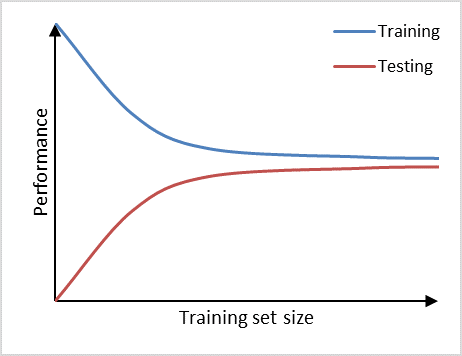
\includegraphics{learningCurve.png}
\caption{Learning curve example.}
\end{figure}

Figure 1, shows an example of learning curve plot in which the vertical
axis represents the model performance and the horizontal axis the
training set size. If training set size is small, the performance on the
training set is high, because a model can often be fitted well to a
limited number of training examples. At the same time, the performance
on the testing set will be poor, because the model trained on such a
limited number of training examples will not generalize well to unseen
data in the testing set. As the training set size increases, the
performance of the model on the training set will decrease. It becomes
more difficult for the model to find a good fit through all the training
examples. Also, the model will be trained on a more representative
portion of training examples, making it generalize better to unseen
data. This can be observed by the increasin testing set performance.

The learning curve can help us in diagnosing bias and variance problems
with our classifier which will provide guidance on how to further
improve our model. We can observe high variance (overfitting) in a
prediction model if it performs well on the training set, but poorly on
the testing set (Figure 2). Adding additional data is a common approach
to counteract high variance. From the learning curve it becomes
apparent, that adding additional data may improve performance on the
testing set a little further, as the learning curve has not yet
plateaued and, thus, the model is not saturated yet. Therefore, adding
more data will decrease the gap between training set and testing set,
which is the main indicator for a high variance problem.

\begin{figure}
\centering
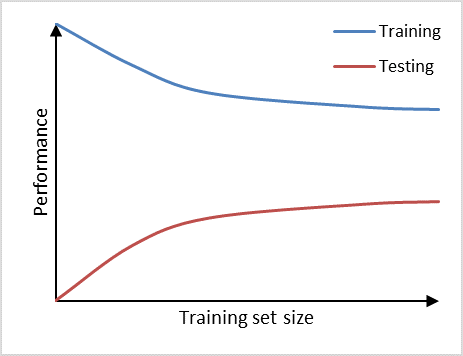
\includegraphics{learningCurveVariance.png}
\caption{Prediction model suffering from high variance.}
\end{figure}

Furthermore, we can observe high bias (underfitting) if a prediction
model performs poorly on the training set as well as on the testing set
(Figure 3). The learning curves of training set and testing set have
flattened on a low performance with only a small gap in between them.
Adding additional data will in this case have little to no impact on the
model performance. Choosing another prediction algorithm that can find
more complex (for example non-linear) relationships in the data may be
an alternative approach to consider in this high bias situation.

\begin{figure}
\centering
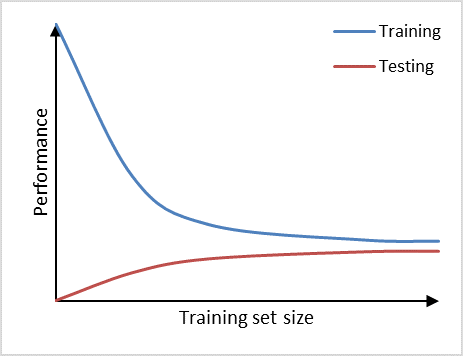
\includegraphics{learningCurveBias.png}
\caption{Prediction model suffering from high bias.}
\end{figure}

\hypertarget{creating-the-learning-curve}{%
\section{Creating the learning
curve}\label{creating-the-learning-curve}}

Use the
\href{http://github.com/OHDSI/PatientLevelPrediction}{\texttt{PatientLevelPrediction}}
package to create a \texttt{population} and \texttt{plpData} object.
Alternatively, you can make use of the data simulator. The following
code snippet creates a population of 12000 patients.

\begin{Shaded}
\begin{Highlighting}[]
\KeywordTok{set.seed}\NormalTok{(}\DecValTok{1234}\NormalTok{)}
\KeywordTok{data}\NormalTok{(plpDataSimulationProfile)}
\NormalTok{sampleSize <-}\StringTok{ }\DecValTok{12000}
\NormalTok{plpData <-}\StringTok{ }\KeywordTok{simulatePlpData}\NormalTok{(}
\NormalTok{  plpDataSimulationProfile,}
  \DataTypeTok{n =}\NormalTok{ sampleSize}
\NormalTok{)}

\NormalTok{population <-}\StringTok{ }\KeywordTok{createStudyPopulation}\NormalTok{(}
\NormalTok{  plpData,}
  \DataTypeTok{outcomeId =} \DecValTok{2}\NormalTok{,}
  \DataTypeTok{binary =} \OtherTok{TRUE}\NormalTok{,}
  \DataTypeTok{firstExposureOnly =} \OtherTok{FALSE}\NormalTok{,}
  \DataTypeTok{washoutPeriod =} \DecValTok{0}\NormalTok{,}
  \DataTypeTok{removeSubjectsWithPriorOutcome =} \OtherTok{FALSE}\NormalTok{,}
  \DataTypeTok{priorOutcomeLookback =} \DecValTok{99999}\NormalTok{,}
  \DataTypeTok{requireTimeAtRisk =} \OtherTok{FALSE}\NormalTok{,}
  \DataTypeTok{minTimeAtRisk =} \DecValTok{0}\NormalTok{,}
  \DataTypeTok{riskWindowStart =} \DecValTok{0}\NormalTok{,}
  \DataTypeTok{riskWindowEnd =} \DecValTok{365}\NormalTok{,}
  \DataTypeTok{verbosity =} \StringTok{"INFO"}
\NormalTok{)}
\end{Highlighting}
\end{Shaded}

Specify the prediction algorithm to be used.

\begin{Shaded}
\begin{Highlighting}[]
\CommentTok{# Use LASSO logistic regression}
\NormalTok{modelSettings <-}\StringTok{ }\KeywordTok{setLassoLogisticRegression}\NormalTok{()}
\end{Highlighting}
\end{Shaded}

Specify a test fraction and a sequence of training set fractions.
Alternatively, you can provide a sequence of training events instead of
the training set fractions. This is recommended, because events are
determinant of model performance. Make sure that your training set can
provide the number of events specified.

\begin{Shaded}
\begin{Highlighting}[]
\NormalTok{testFraction <-}\StringTok{ }\FloatTok{0.2}
\NormalTok{trainFractions <-}\StringTok{ }\KeywordTok{seq}\NormalTok{(}\FloatTok{0.1}\NormalTok{, }\FloatTok{0.8}\NormalTok{, }\FloatTok{0.1}\NormalTok{) }\CommentTok{# Create eight training set fractions}

\CommentTok{# alternatively use a sequence of training events by uncommenting the line below.}
\CommentTok{# trainEvents <- seq(100, 5000, 100)}
\end{Highlighting}
\end{Shaded}

Specify the test split to be used.

\begin{Shaded}
\begin{Highlighting}[]
\CommentTok{# Use a split by person, alternatively a time split is possible}
\NormalTok{testSplit <-}\StringTok{ 'stratified'}
\end{Highlighting}
\end{Shaded}

Create the learning curve object.

\begin{Shaded}
\begin{Highlighting}[]
\NormalTok{learningCurve <-}\StringTok{ }\KeywordTok{createLearningCurve}\NormalTok{(population,}
                                     \DataTypeTok{plpData =}\NormalTok{ plpData,}
                                     \DataTypeTok{modelSettings =}\NormalTok{ modelSettings,}
                                     \DataTypeTok{testFraction =} \FloatTok{0.2}\NormalTok{,}
                                     \DataTypeTok{verbosity =} \StringTok{"TRACE"}\NormalTok{,}
                                     \DataTypeTok{trainFractions =}\NormalTok{ trainFractions,}
                                     \CommentTok{# trainEvents = trainEvents,}
                                     \DataTypeTok{splitSeed =} \DecValTok{1000}\NormalTok{,}
                                     \DataTypeTok{saveModel =} \OtherTok{TRUE}\NormalTok{)}
\end{Highlighting}
\end{Shaded}

Plot the learning curve object (Figure 4). Specify one of the available
metrics: \texttt{AUROC}, \texttt{AUPRC}, \texttt{sBrier}. Moreover, you
can specify what metric to put on the abscissa, number of
\texttt{observations} or number of \texttt{events}. We recommend the
latter, because \texttt{events} are determinant of model performance and
allow you to better compare learning curves across different prediction
problems and databases.

\begin{Shaded}
\begin{Highlighting}[]
\KeywordTok{plotLearningCurve}\NormalTok{(}
\NormalTok{  learningCurve,}
  \DataTypeTok{metric =} \StringTok{'AUROC'}\NormalTok{,}
  \DataTypeTok{abscissa =} \StringTok{'events'}\NormalTok{,}
  \DataTypeTok{plotTitle =} \StringTok{'Learning Curve'}\NormalTok{,}
  \DataTypeTok{plotSubtitle =} \StringTok{'AUROC performance'}
\NormalTok{)}
\end{Highlighting}
\end{Shaded}

\begin{figure}
\centering
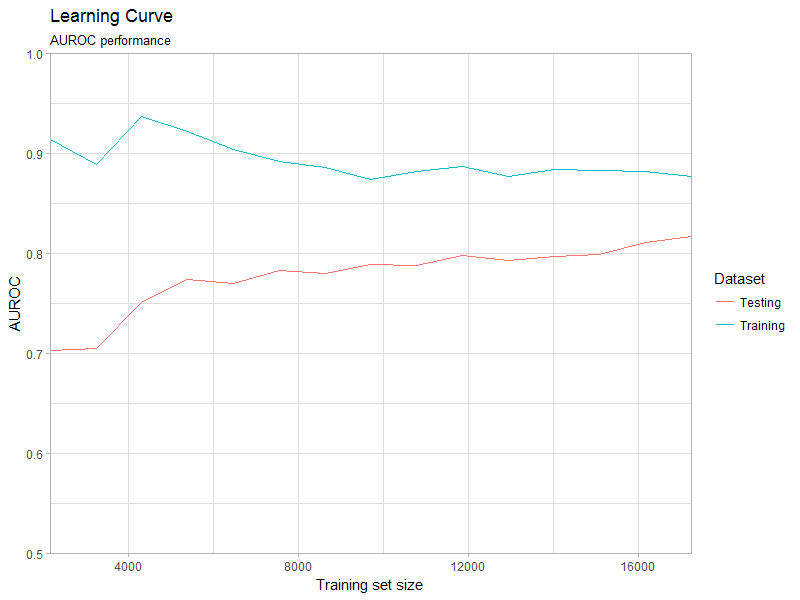
\includegraphics{learningCurvePlot.png}
\caption{Learning curve plot.}
\end{figure}

\hypertarget{parallel-processing}{%
\section{Parallel processing}\label{parallel-processing}}

The learning curve object can be created in parallel, which can reduce
computation time significantly. Currently this functionality is only
available for LASSO logistic regression and gradient boosting machines.
Depending on the number of parallel workers it may require a significant
amount of memory. We advise to use the parallelized learning curve
function for parameter search and exploratory data analysis.

Use the parallelized version of the learning curve function to create
the learning curve object in parallel. R will find the number of
available processing cores automatically and register the required
parallel backend. Alternatively, you can provide the number of cores you
wish to use.

\begin{Shaded}
\begin{Highlighting}[]
\NormalTok{learningCurvePar <-}\StringTok{ }\KeywordTok{createLearningCurvePar}\NormalTok{(}
\NormalTok{  population,}
  \DataTypeTok{plpData =}\NormalTok{  plpData,}
  \DataTypeTok{modelSettings =}\NormalTok{ modelSettings,}
  \DataTypeTok{testSplit =}\NormalTok{ testSplit,}
  \DataTypeTok{testFraction =}\NormalTok{ testFraction,}
  \DataTypeTok{trainEvents =}\NormalTok{ trainEvents,}
  \DataTypeTok{cores =} \DecValTok{4}\NormalTok{,}
  \DataTypeTok{splitSeed =} \DecValTok{1000}
\NormalTok{)}
\end{Highlighting}
\end{Shaded}

\hypertarget{demo}{%
\section{Demo}\label{demo}}

We have added a demo of the learningcurve:

\begin{Shaded}
\begin{Highlighting}[]
\CommentTok{# Show all demos in our package: }
 \KeywordTok{demo}\NormalTok{(}\DataTypeTok{package =} \StringTok{"PatientLevelPrediction"}\NormalTok{)}

\CommentTok{# Run the learning curve}
 \KeywordTok{demo}\NormalTok{(}\StringTok{"LearningCurveDemo"}\NormalTok{, }\DataTypeTok{package =} \StringTok{"PatientLevelPrediction"}\NormalTok{)}
\end{Highlighting}
\end{Shaded}

Do note that running this demo can take a considerable amount of time
(15 min on Quad core running in parallel)!

\hypertarget{publication}{%
\section{Publication}\label{publication}}

A publication titled `How little data do we need for patient-level
prediction?' uses the learning curve functionality in this package and
can be accessed as preprint in the arXiv archives at
\url{https://arxiv.org/abs/2008.07361}.

\hypertarget{acknowledgments}{%
\section{Acknowledgments}\label{acknowledgments}}

Considerable work has been dedicated to provide the
\texttt{PatientLevelPrediction} package.

\begin{Shaded}
\begin{Highlighting}[]
\KeywordTok{citation}\NormalTok{(}\StringTok{"PatientLevelPrediction"}\NormalTok{)}
\end{Highlighting}
\end{Shaded}

\begin{verbatim}
## 
## To cite PatientLevelPrediction in publications use:
## 
## Reps JM, Schuemie MJ, Suchard MA, Ryan PB, Rijnbeek P (2018). "Design and implementation of a standardized framework
## to generate and evaluate patient-level prediction models using observational healthcare data." _Journal of the
## American Medical Informatics Association_, *25*(8), 969-975. <URL: https://doi.org/10.1093/jamia/ocy032>.
## 
## A BibTeX entry for LaTeX users is
## 
##   @Article{,
##     author = {J. M. Reps and M. J. Schuemie and M. A. Suchard and P. B. Ryan and P. Rijnbeek},
##     title = {Design and implementation of a standardized framework to generate and evaluate patient-level prediction models using observational healthcare data},
##     journal = {Journal of the American Medical Informatics Association},
##     volume = {25},
##     number = {8},
##     pages = {969-975},
##     year = {2018},
##     url = {https://doi.org/10.1093/jamia/ocy032},
##   }
\end{verbatim}

\textbf{Please reference this paper if you use the PLP Package in your
work:}

\href{http://dx.doi.org/10.1093/jamia/ocy032}{Reps JM, Schuemie MJ,
Suchard MA, Ryan PB, Rijnbeek PR. Design and implementation of a
standardized framework to generate and evaluate patient-level prediction
models using observational healthcare data. J Am Med Inform Assoc.
2018;25(8):969-975.}

\end{document}
